\section{Unfairness of Atomic Swaps}
\label{sec:evaluation}

Recall that the premium is the price paid by the option buyer for signing the option contract with the option seller.
In the Atomic Swap, Alice is not required to pay for the premium.
In this way, Alice can decide whether to proceed the swap while investigating the cryptocurrency market.
This enables Alice to speculate without any risk:
if Alice's asset price rises right before the strike time, he will proceed the swap to profit, otherwise he will abort the swap to avoid the loss.
Therefore, without the premium, Alice is risk-free towards the market.

In this section, we evaluate the unfairness of the Atomic Swap based on our formalization in Section~\ref{sec:formalization}.
In particular, we evaluate the unfairness from two perspectives: quantifying the unfairness and estimating the unpaid premium.
Quantifying the unfairness is based on analyzing the historical exchange rate volatility, while estimating the unpaid premium is based on the Cox-Ross-Rubinstein option pricing model - the conventional option pricing model for American-style options.
Furthermore, we also evaluate conventional financial assets - the stocks and the currency exchanges - and compare their results with cryptocurrencies.

\subsection{Experimental setting}

We collected relevant data of mainstream cryptocurrencies for one year, starting from May 3th, 2018 to May 3th, 2019.
In particular, the cryptocurrency exchange rate data was retrieved from from CoinGecko~\footnote{\url{https://www.coingecko.com}. Data was fetched at May 4th, 2019.};
the stock index data was retrieved from Yahoo Finance~\footnote{\url{https://finance.yahoo.com}. Data was fetched at May 4th, 2019.};
the currency exchange rate data was retrieved from Investing.com~\footnote{\url{https://www.investing.com}. Data was fetched at May 4th, 2019.}.

All experiments run on a MacBook Pro with a 2.2 GHz Intel Core i7 Processor, a 16 GB DDR4 RAM and 256 SSD storage disk.

\subsection{Quantifying the unfairness by market volatility}
\label{subsec:volatility_analysis}

The unfairness consists of two parts, namely the profit and the mitigated loss from Alice's perspective.
When Bob's asset price rises, Alice profits directly.
When Bob's asset price drops, Alice can abort the swap and transfer the loss to Bob.


Assume that Alice initiates the swap by triggering \textbf{Initiate}($\cdot$) at the time $t$, then by default $\delta_1 = t + 48 (\text{hours})$.
We also assume that Bob participates in the swap by triggering \textbf{Participate}($\cdot$), then by default $\delta_2 = t + 24 (\text{hours})$.
In this way, Alice can decide whether to proceed the swap within $ \delta_1 - \delta_2 = 24 (\text{hours})$.

We test the unfairness by using a single Atomic Swap with the value of $x$ USD, then we show the degree of unfairness in dollars based on the historical data.
For each day, Alice may either profit $\alpha$ percent of $x$ directly (when Bob's asset price rises),
or mitigate $\beta$ percent of $x$ by aborting the swap (when Bob's asset price drops) on average.
Assume the possibility for Bob's asset price to rise is $P_{\alpha}$, and to drop is $P_{\beta}$.
Then, the expected profit rate is $E_{\alpha} = \alpha P_{\alpha}$,
and the expected mitigated risk rate is $E_{\beta} = \beta P_{\beta}$.
Therefore, the expected unfairness is that Alice profits $E_{\alpha} x$ and mitigates the risk of losing $E_{\beta} x$.
Also, as $E_\alpha$ and $E_\beta$ are equally calculated, they can be added together to derive the total unfairness as $E_\alpha + E_\beta$.

\paragraph{Experimental methodology.}
In our scenario, quantifying the unfairness is to estimate $E_{\alpha}$ and $E_{\beta}$.
We estimate $E_{\alpha}$ and $E_{\beta}$ for each selected cryptocurrency pair.
Furthermore,  we also evaluate the unfairness of stocks and fiat currencies in the same setting, in order to make comparisons.
We use S\&P500 and Dow Jones Index (DJI) as examples of stocks, and USD-EUR and USD-GBP as examples of fiat currencies.

\paragraph{Results and analysis.}

\begin{figure*}
    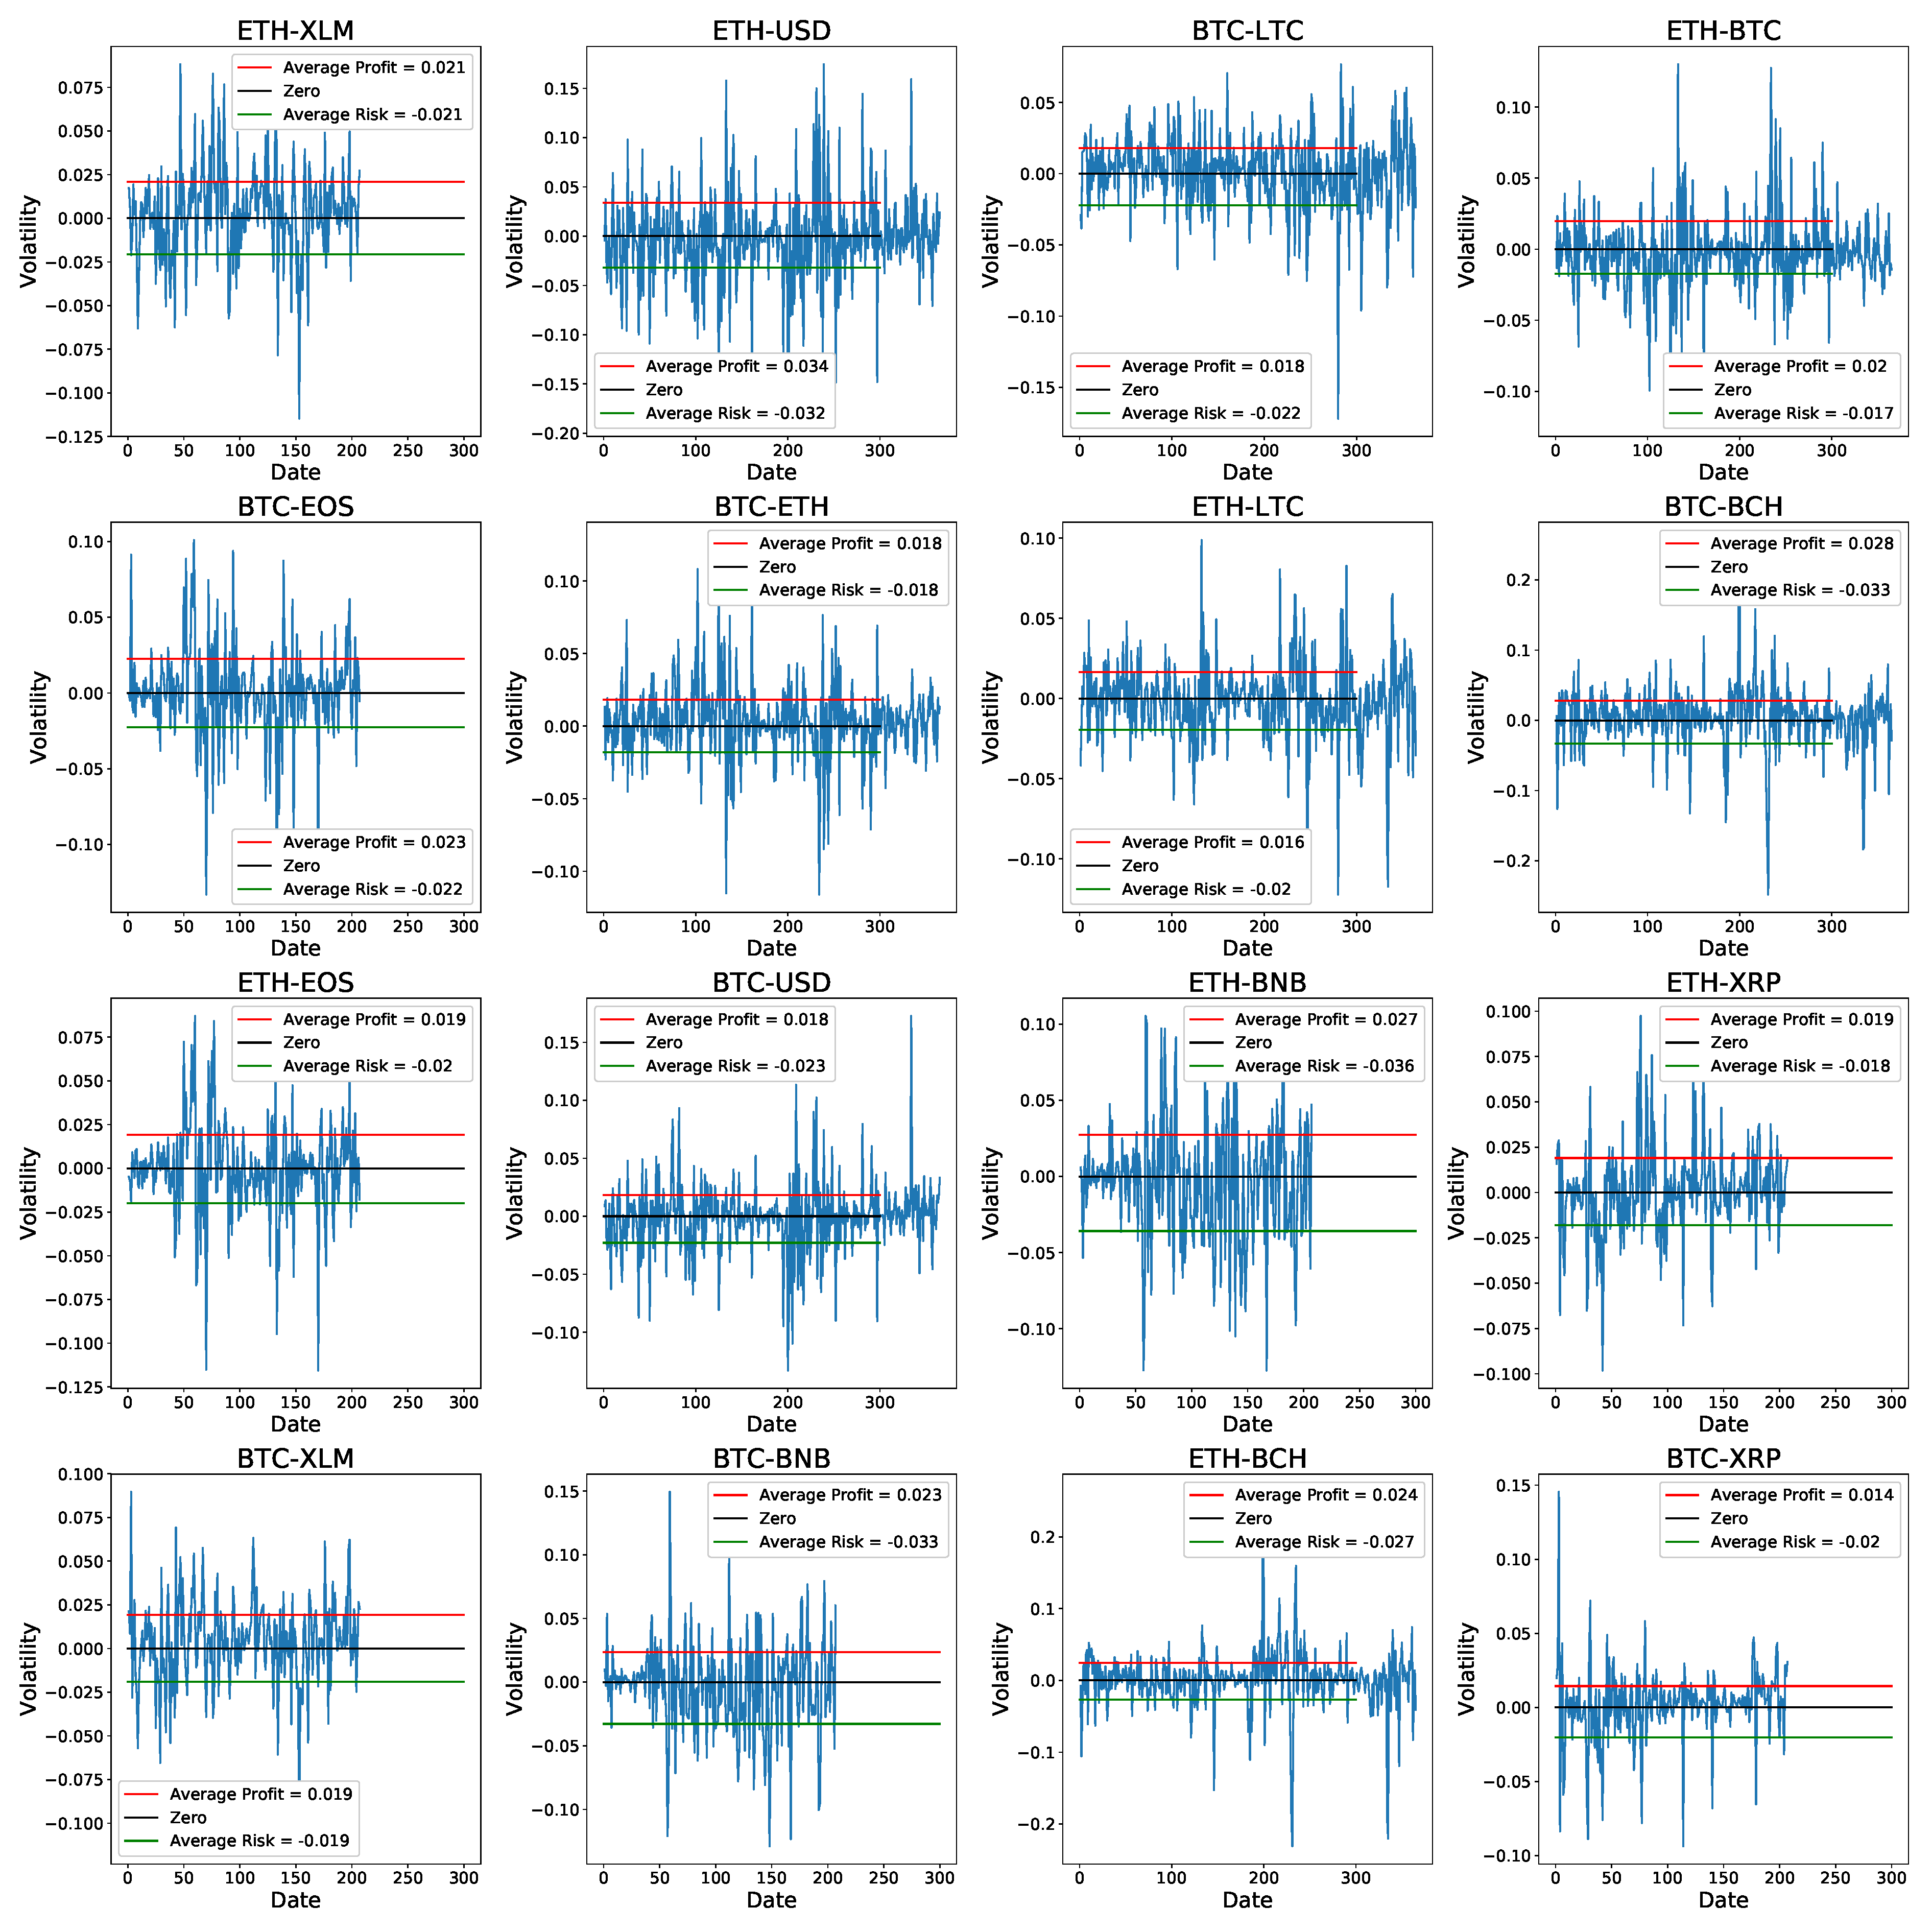
\includegraphics[width=\linewidth]{volatility_analysis.eps}
    \caption{The daily percentage changes for all selected cryptocurrency pairs, stock indices and fiat currency pairs over one year (from 03/05/2018 to 03/05/2019). For each figure, $E_{\alpha}$, $E_{\beta}$, $max_\alpha$ and $max_\beta$ are the expected profit rate, the expected mitigated risk rate, the maximum daily profit and the maximum daily mitigated risk, respectively.}
    \label{fig:volatility_analysis}
\end{figure*}

\begin{figure}
    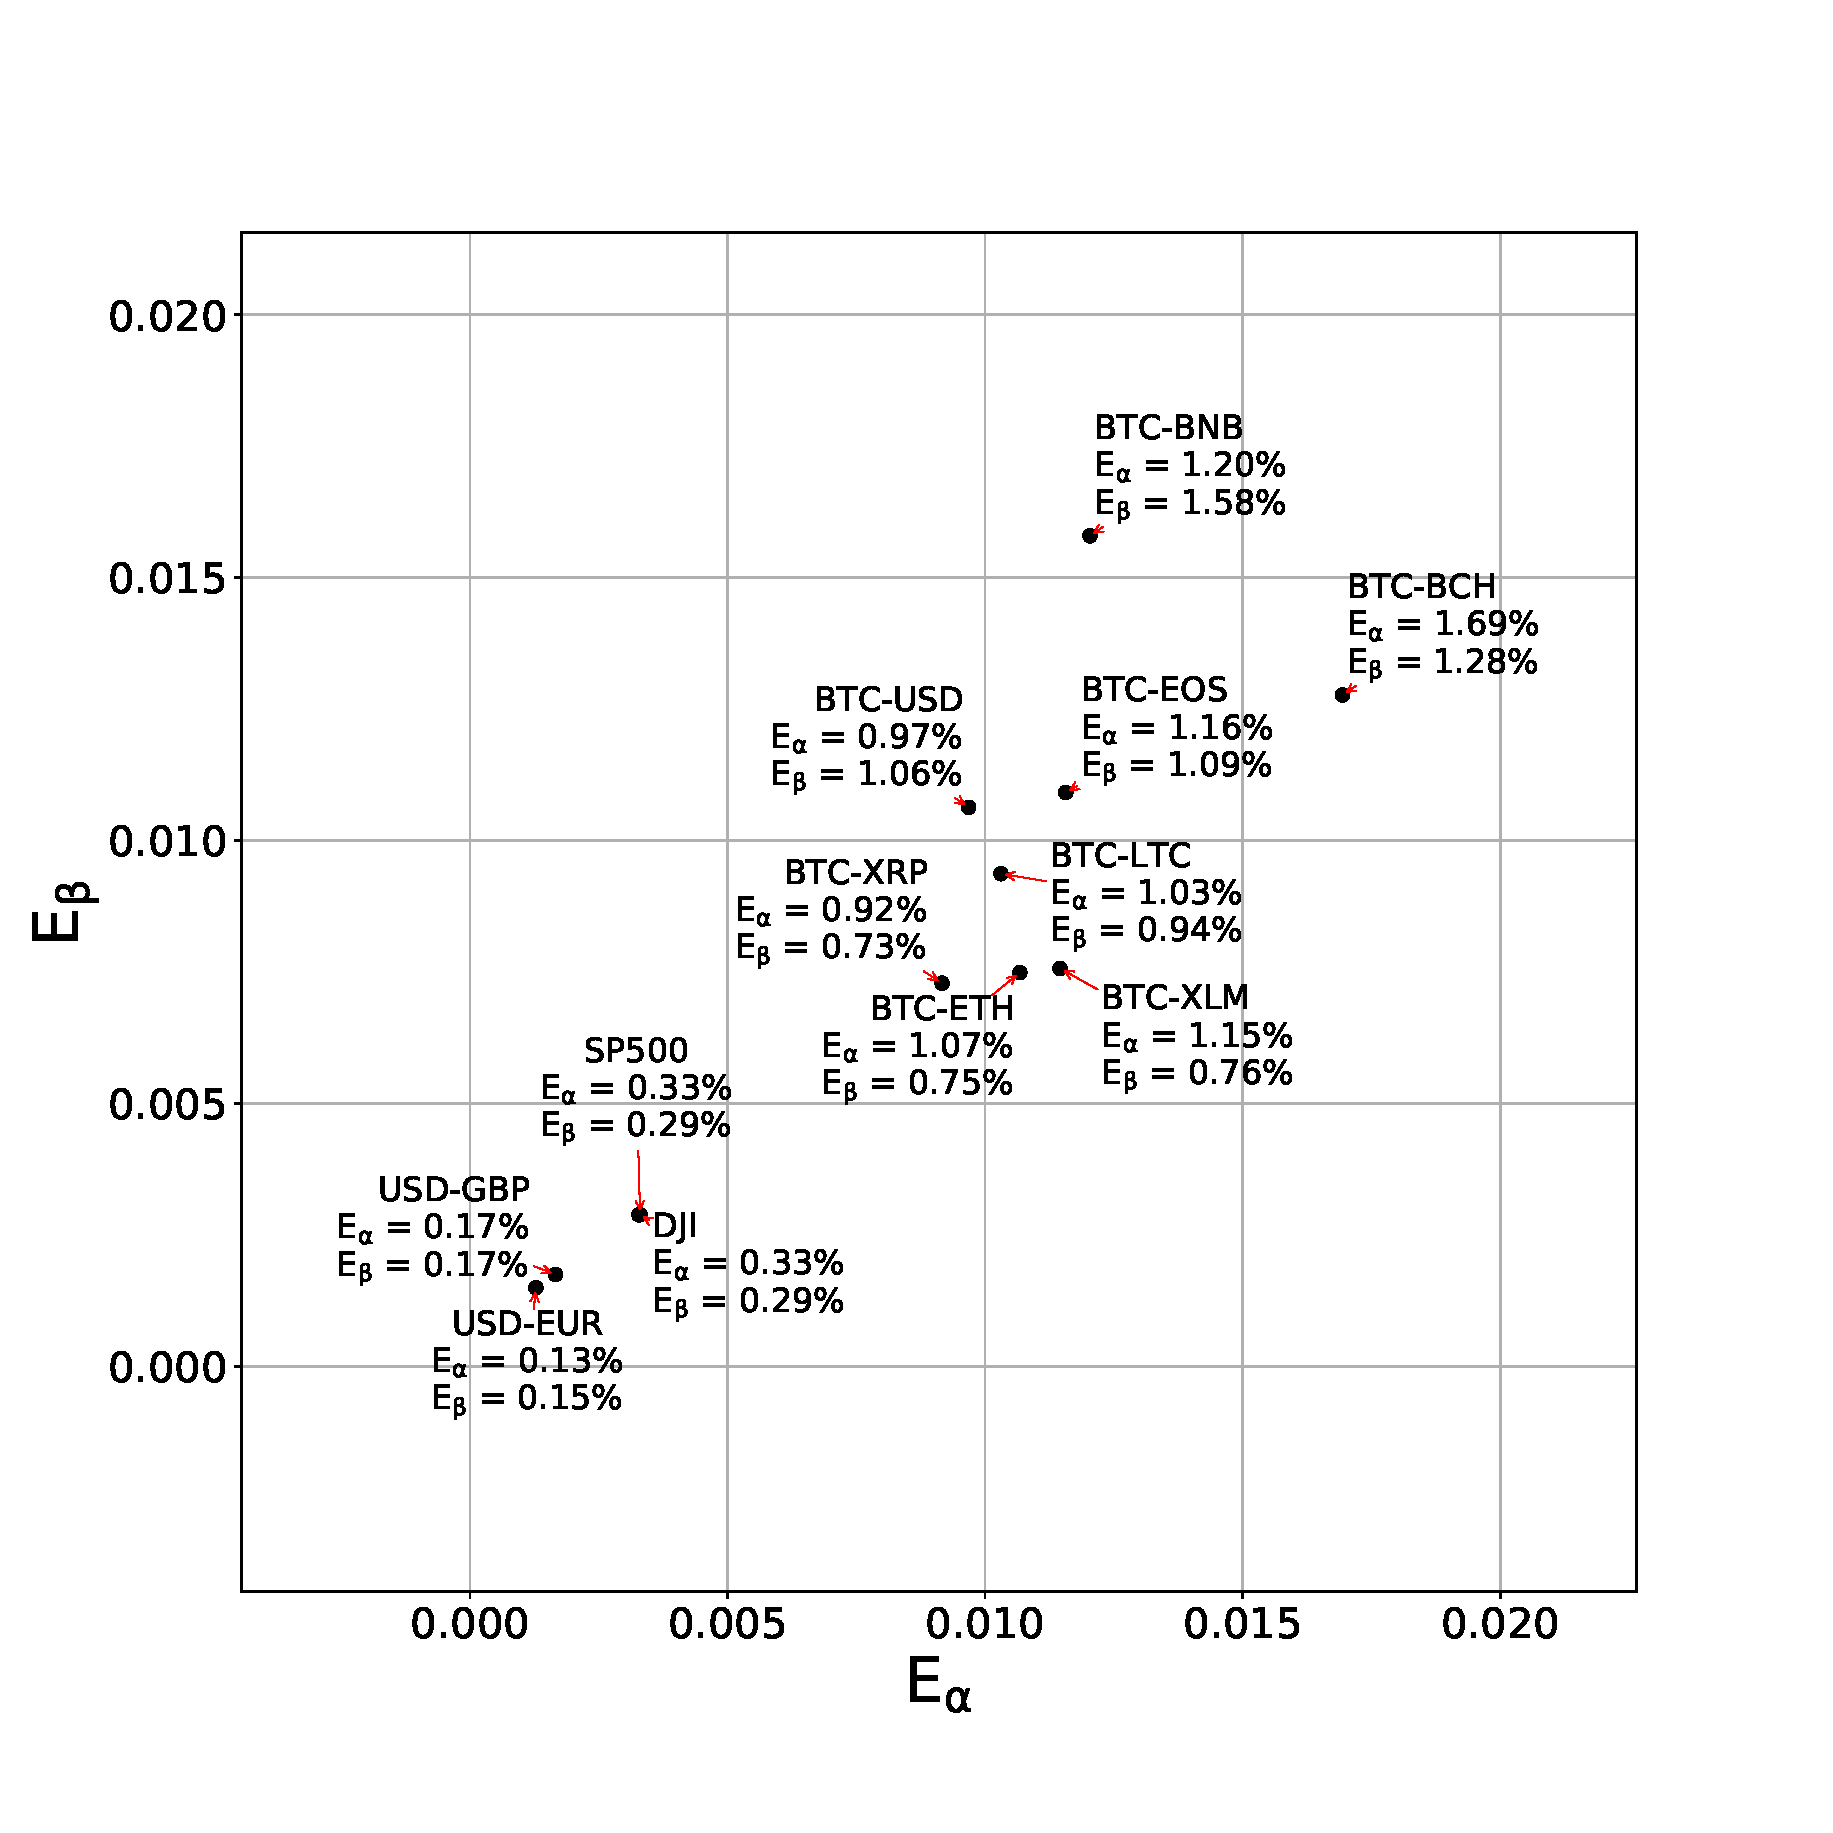
\includegraphics[width=\linewidth]{vol_scatter.eps}
    \caption{Visualizing the expected profit rate $E_\alpha$ and the expected mitigated risk rate $E_\beta$ for each cryptocurrency pair, stock index and fiat currency pair.}
    \label{fig:vol_scatter}
\end{figure}

% line analysis
Figure~\ref{fig:volatility_analysis} shows the estimated $E_\alpha$, $E_\beta$, the maximum daily rises $max_\alpha$ and the maximum daily drops $max_\beta$ for chosen 8 cryptocurrency pairs, stock indices (S\&P500 and DJI) and fiat currency exchange rates (USD-EUR and USD-GBP).
For each plot, points in the red Profit Area indicate that Alice profits directly at those days, and points in the green Risk Area indicate that Alice will abort the swap to mitigate the risk.

We observe that for all chosen cryptocurrency pairs, $max_\alpha$ and $max_\beta$ are quite big - ranging from 8\% to 25\%.
Meanwhile, $max_\alpha$ and $max_\beta$ of stock indices are much smaller than all cryptocurrency pairs,
and $max_\alpha$ and $max_\beta$ of fiat currencies are even smaller than stock indices.
This indicates that in the setting of an 24-hour Atomic Swap, the cryptocurrency is much more unfair than stocks, and the stocks are more unfair than fiat currencies.


% scatter results and analysis
Figure~\ref{fig:vol_scatter} visualizes $E_\alpha$ and $E_\beta$ of all evaluated items in Figure~\ref{fig:volatility_analysis}.
In particular, we classify scatters to 4 groups based on their $E_\alpha$ and $E_\beta$:
The first group ($E_\alpha < 0.005 \wedge E_\beta < 0.005$) consists of all stocks and fiat currency pairs (S\&P500, DJI, USD-GBP and USD-EUR);
the second group ($0.005 < E_\alpha < 0.015 \wedge 0.005 < E_\beta < 0.015$) consists of most cryptocurrency pairs;
the third group ($0.005 < E_\alpha < 0.015 \wedge E_\beta > 0.015$) only contains one cryptocurrency pair BTC-BNB;
the fourth group ($E_\alpha > 0.015 \wedge 0.005 < E_\beta < 0.015$) only contains the last cryptocurrency pair BTC-BCH.
Moreover, we draw a line $E_\beta = E_\alpha$ to separate two areas: $E_\beta > E_\alpha$ and $E_\beta < E_\alpha$.

Obviously, the Atomic Swap with first-group items is fairer than with second-group items, and the Atomic Swap with second-group items is fair than with third-group and fourth-group items.
Therefore, we can get the following results.
First, the Atomic Swap with cryptocurrency pairs is more unfair than with stocks and fiat currency pairs. This result is consistent with results in Figure~\ref{fig:volatility_analysis}.
Second, $E_\beta$ and $E_\beta - E_\alpha$ of BTC-BNB are bigger than of others. This means the exchange rate of BTC-BNB drops generally over the last year.
Meanwhile, $E_\alpha$ and $E_\alpha - E_\beta$ of BTC-BCH are bigger than of others. This means the exchange rate of BTC-BCH rises generally over the last year.
Both observations indicate that BTC-BNB and BTC-BCH are highly volatile, so the Atomic Swap with those assets is more unfair than with other assets.
Third, all dots are close to the line $E_\beta = E_\alpha$, while the dots of stocks and fiat currency pairs almost lay on this line.
A dot lying on $E_\beta = E_\alpha$ means the exchange rate rises and drops at the same level.
Therefore, although more volatile than stocks and fiat currency pairs, exchange rates of cryptocurrency pairs rise and drop at the same level.
















\subsection{Estimating the premium}

The unfairness of the Atomic Swap comes from the fact that Alice can abort the contract without punishment.
In Finance, the premium mechanism guarantees the good behaviours, which also works for Atomic Swaps.
Therefore, we can evaluate the unfairness of the Atomic Swap by estimating the premium for American Call Options with cryptocurrencies.

As the premium is the only variable in an option contract, estimating the premium is also called the ``Option Pricing'' problem.
In Finance, the Black-Scholes (BS) Model is utilized to price the European Call Options,
while the Cox-Ross-Rubinstein (CRR) Model is utilized to price the American Call Options.

Therefore, in order to evaluate the unfairness of the Atomic Swap, we utilize the CRR Model to estimate the premium for American Call Options with cryptocurrencies.

\subsubsection{The Cox-Ross-Rubinstein Model Explained}

The Cox-Ross-Rubinstein (CRR) Model~\cite{cox1979option} - a.k.a. the Binomial Options Pricing Model (BOPM) - provides a generalizable numerical method for pricing the options.
Intuitively, the CRR model enumerates all possible prices of the asset in the near future based on the price volatility,
then reverse-engineers the premium based on the enumerated prices.
% binomial tree
The model assume that for each step on the binomial tree, the asset price rises or falls by a fixed rate.
Enumerating the possible asset prices constructs a binomial tree, where each node attaches an asset price and a premium price at a point of time.
% reverse engineering
By iteratively back propagating the premium from the leaves to the root of the binomial tree, the premium will be revealed.

Formally, using the CRR model to price the American Call Option $\Pi = (\pi_1, \pi_2, K, A, T, C)$ with the underlying price $S_t$ of $\pi_2$ follows the steps below:
\begin{enumerate}
    \item Creating the binomial price tree
    \item Calculating the premiums for leaf nodes
    \item Iteratively reconstructing the premiums for non-leaf nodes 
\end{enumerate}

\begin{figure}
\centering
\begin{tikzpicture}[
    >=stealth,
    sloped,
    draw=black,thick,anchor=west,
    scale=0.8,
    every node/.style={scale=0.8}
]
\matrix (tree) [%
    matrix of nodes,
    minimum size=1cm,
    column sep=1.4cm,
    row sep=0.5cm,
]
{
               &                                         & $S_{\frac{2T}{n}, 1} = u^2 \cdot S_{0, 1}$ \\
               & $S_{\frac{T}{n}, 1} = u \cdot S_{0, 1}$ &   \\
    $S_{0, 1}$ &                                         & $S_{\frac{2T}{n}, 2} = S_{0, 1}$ \\
               & $S_{\frac{T}{n}, 2} = d \cdot S_{0, 1}$ &   \\
               &                                         & $S_{\frac{2T}{n}, 3} = d^2 \cdot S_{0, 1}$ \\
};
\draw[->] (tree-3-1) -- (tree-2-2) node [midway,above] {$p$};
\draw[->] (tree-3-1) -- (tree-4-2) node [midway,below] {$(1-p)$};
\draw[->] (tree-2-2) -- (tree-1-3) node [midway,above] {$P^2$};
\draw[->] (tree-2-2) -- (tree-3-3) node [midway,below] {$(1-p)p$};
\draw[->] (tree-4-2) -- (tree-3-3) node [midway,above] {$(1-p)p$};
\draw[->] (tree-4-2) -- (tree-5-3) node [midway,below] {$(1-p)^2$};
\end{tikzpicture}
\caption{The binomial price tree $\mathcal{T}$.}
\label{fig:binomial_tree}
\end{figure}


\paragraph{Creating the binomial price tree.}
The binomial price tree $\mathcal{T}$ of the height $n$ represents the possible future prices within the time period $T$ discretely, as shown in Fig.~\ref{fig:binomial_tree}.
$n$ can be picked arbitrarily. With larger $n$, the result will be more accurate, but the computing overhead will be heavier.
Each node $\mathcal{T}_{t, i}$ is attached with the asset price $S_{t, i}$ and the premium $C_{t, i}$,
where $t \in \{0, \frac{T}{n}, \frac{2T}{n}, \dots, T\}$ is the point of time and $i$ is the number of the node at its level.
The CRR model assumes that the asset price will either move up or down by a specific factor per step in $\mathcal{T}$.
The move-up factor is $u$, and the move-down factor is $d$.
For example, given the initial asset price $S_{0, 1}$, the asset price after one move-up $S_{\frac{T}{n}, 1}$ is $u \cdot S_{0, 1}$, and the asset price after one move-down $S_{\frac{T}{n}, 2}$ is $d \cdot S_{0, 1}$.

$u$ and $d$ are calculated using the annualized volatility $\sigma_a$ of the underlying asset price.
In the CRR model, the move-up and move-down are symmetric - $u \cdot d = 1$, and the rate of move-up and move-down is positive correlated with $\sigma_a$:

\begin{align} 
u &= e^{\sigma_a \sqrt{\frac{T}{n}}}\\
d &= e^{- \sigma_a \sqrt{\frac{T}{n}}} = \frac{1}{u}
\end{align}

Here, $T$ is measured in years, and $\sigma_a$ is defined as the standard deviation of the annual price.
$\sigma_a$ can be computed from the daily price standard deviation $\sigma_d$ as below:

\begin{align} 
\sigma_a &= \sigma_d \sqrt{d}\\
\sigma_d &= \sqrt{\frac{\sum^{d}_{i=1} (S_i - \bar{S})^2}{d-1}}
\end{align}

where $d$ is the number of trading days within a year.
For cryptocurrencies, $d$ equals to the number of a days within a year.
Note that $S_i$ is the percentage change of the price on day $i$, rather than the price itself.
$\bar{S}$ is the average value of all $S_i$s within the $d$ days. 

The asset price $S_{t, i}$ can also be computed as $S_{t, i} = S_{0, 1} \cdot u^{N_u - N_d}$, where $S_{0, 1}$ is the spot price, and $N_u, N_d$ are the numbers of move-up and move-down, respectively.

\paragraph{Calculating the premiums for leaf nodes.}
In the first step, only the asset prices are determined rather than the premiums.
This step further determines the premiums for leaf nodes.
For each leaf node $\mathcal{T}_{n, i}$, the premium (for Call Options) is $C_{n, i} = max[(S_{n, i} - K), 0]$.

\paragraph{Iteratively reconstructing the premiums for earlier nodes.}
We back-propagate the premiums for leaf nodes to earlier premiums.
More specifically, the earlier premium is calculated from the premiums of the later two nodes weighted by their state transition possibilities.
The move-up and move-down possibility are $p$ and $q$ where $p + q = 1$, and the risk-free rate is $r = q$.

The earlier premium $C_{t - \Delta t, i}$ is calculated from later premiums as:

\begin{align}
C_{t - \Delta t, i} = e^{-r \Delta t} (p C_{t, i} + q C_{t, i+1})
\end{align}

where $\Delta t = \frac{T}{n}$, and $p, q, r$ are computed as

\begin{align} 
p &= \frac{e^{(r-q)\Delta t} - d}{u - d}\\
q &= 1 - p\\
r &= q
\end{align}

such that the premium distribution simulates the geometric Brownian motion with parameters $r$ and $\sigma$.

The earliest premium $S_{0, 1}$ - the estimated premium - can be calculated by iteratively back-propagating the later premiums. 

\JS{A table summarizing the notations will be nice — there are too many different notations, and I cannot remember them all. (added by Runchao)}

\subsubsection{Experiments}


\begin{figure}
    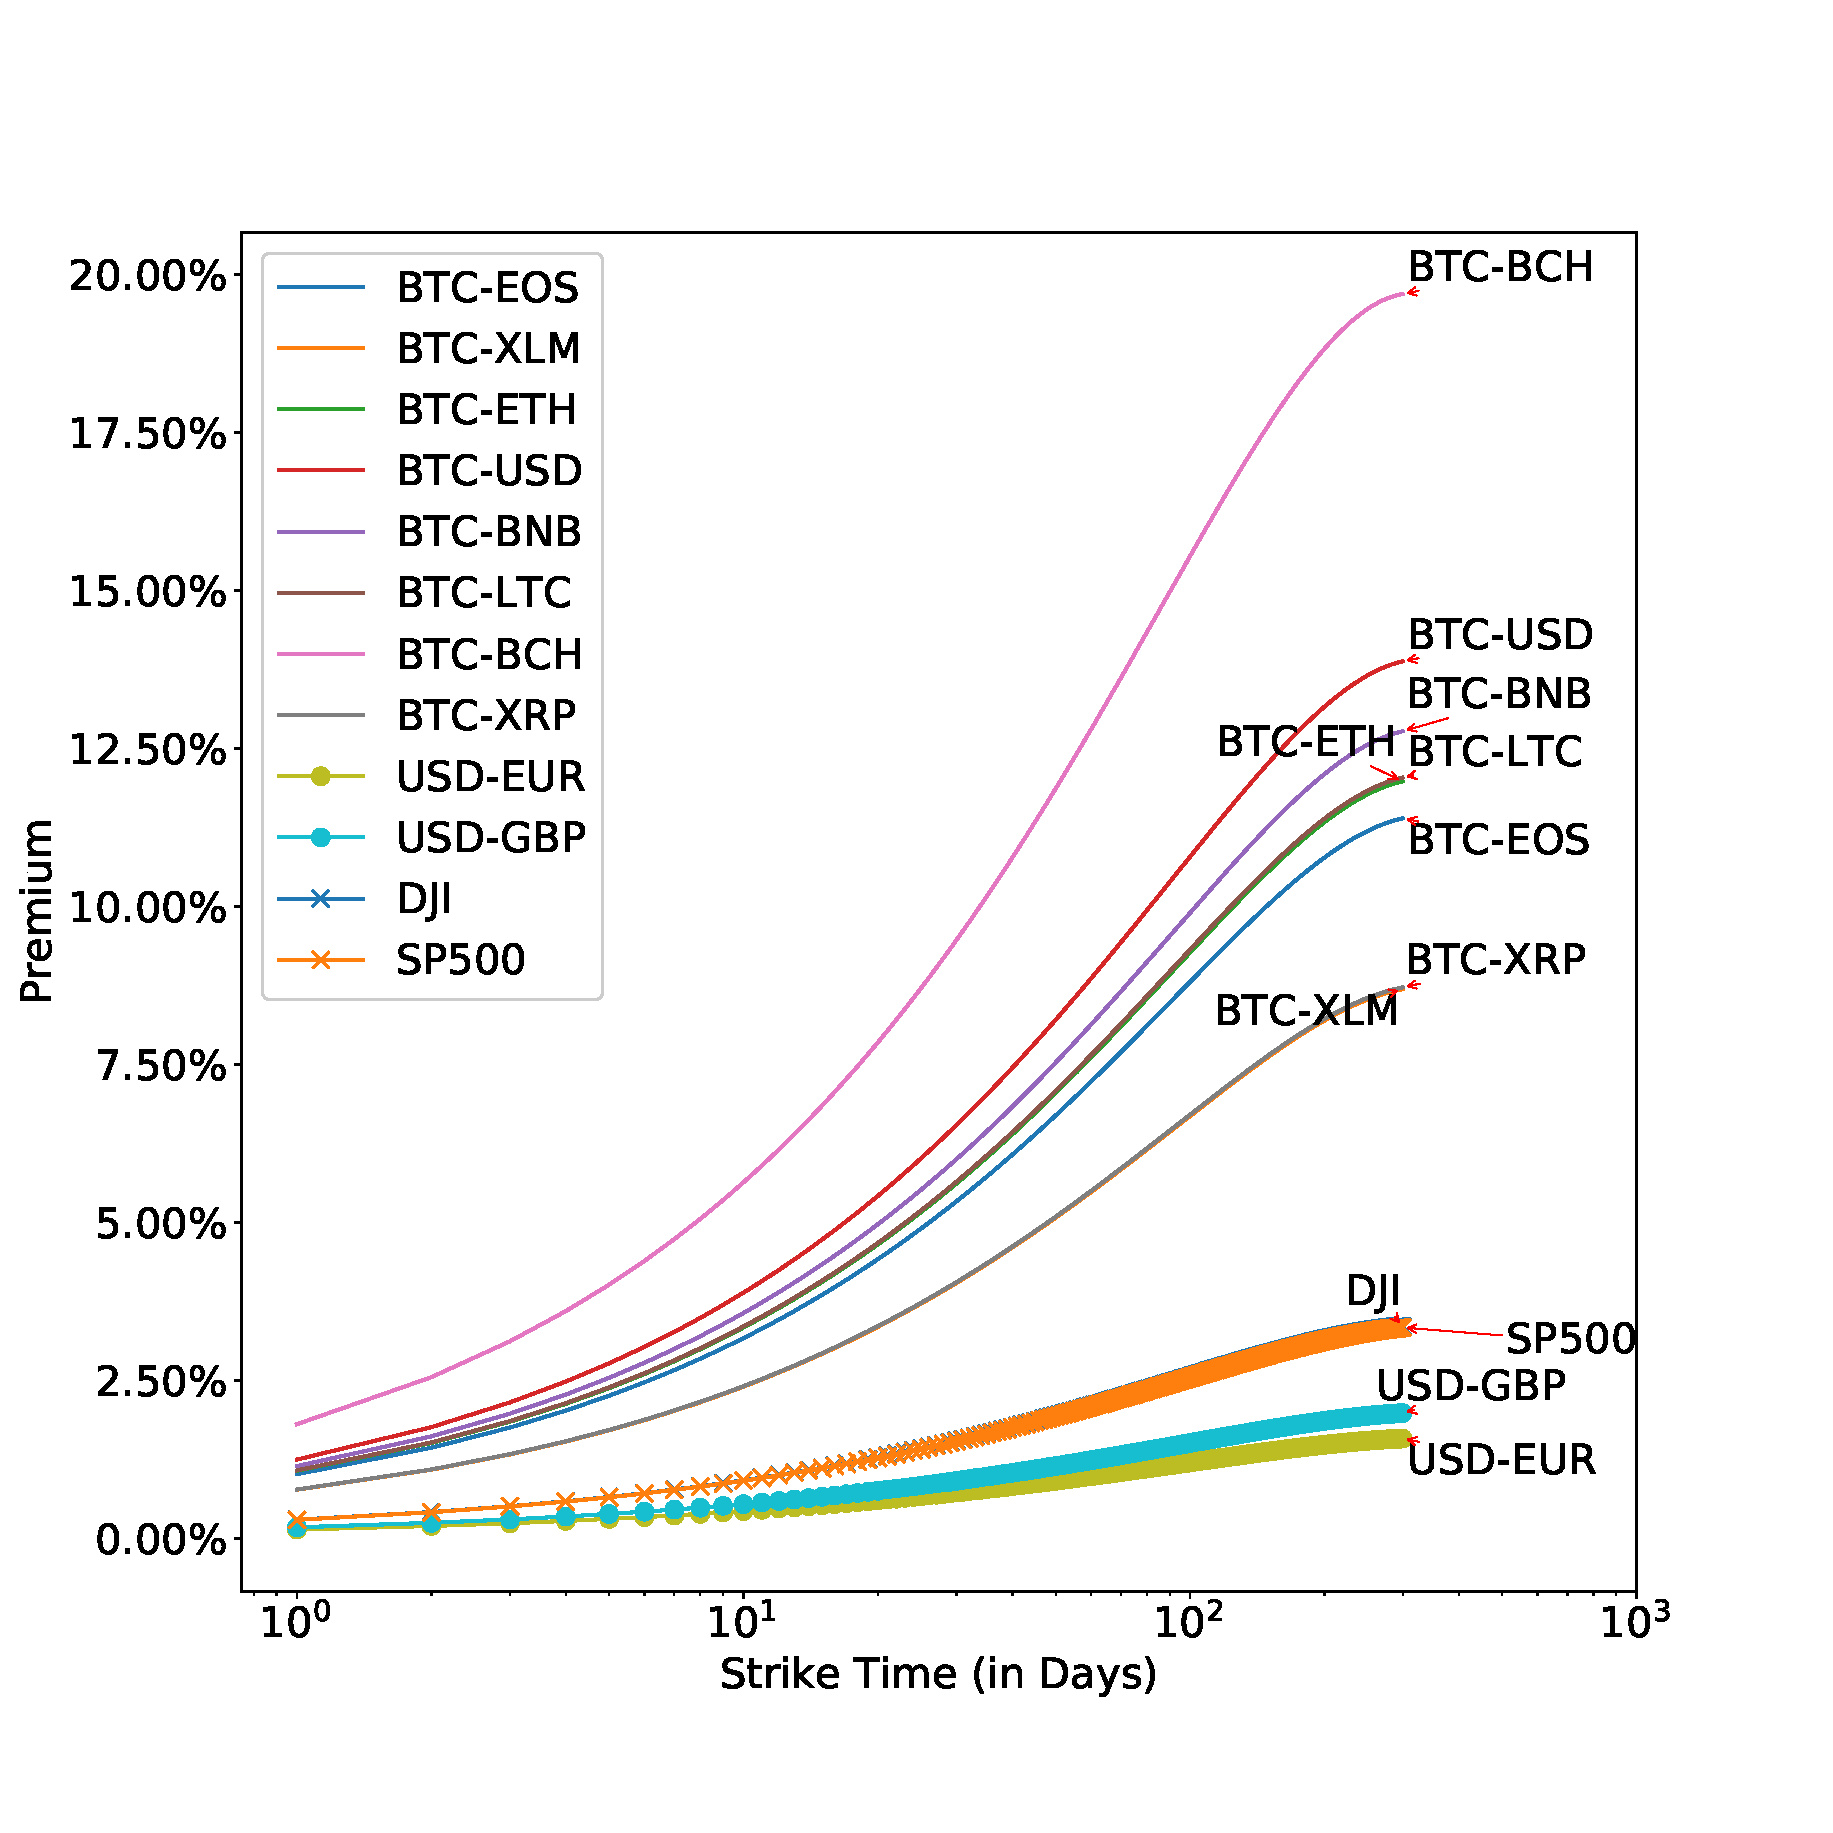
\includegraphics[width=\linewidth]{premium_pricing_result.eps}
    \caption{Estimated premium with different strike times for each cryptocurrency pair, stock index and fiat currency pair. Lines with the marker ``x'' are for stocks; lines with the marker ``o'' are for fiat currencies; and lines without marker are for cryptocurrency pairs.}
    \label{fig:premium_pricing_result}
\end{figure}

We price the same data as Section~\ref{subsec:volatility_analysis} by using the CRR model with $n = 36$ with the strike time $T$ ranging from $1$ to $300$.
Figure~\ref{fig:premium_pricing_result} shows our pricing results.

First, we observe that the premium of cryptocurrency pairs is much more expensive than stocks, and the premium of stocks is more expensive than fiat currencies at any given time.
Recall the evaluated unfairness in Section~\ref{subsec:volatility_analysis}, its results are consistent with the premium pricing results: The higher the volatility is, the more unfair the Atomic Swap will be, and the higher the premium should be.

Second, with the default strike time $T = 1$ of the Atomic Swap, the premium of cryptocurrency pairs vary from approximately 1\% to 2.3\% of the underlying asset value.

Third, for all evaluated items, the premium values rise monotonically.
This is because the longer expiration time lets the option buyer to have more control on the option - He has more time to predict the price and judges whether to exercise the option.